% Academic preprint. This manuscript is independent of a workshop template.
\documentclass[10pt,twocolumn,letterpaper]{article}
\usepackage{cvpr}
\usepackage{booktabs}
\usepackage{graphicx}
\usepackage{multirow}
\usepackage{amsmath}
\usepackage{array}
\usepackage{tabularx}
\usepackage{xcolor}
\usepackage{listings}
\usepackage{placeins}
\usepackage{balance}
\usepackage{url}

\let\originalthebibliography\thebibliography
\renewcommand{\thebibliography}[1]{%
  \originalthebibliography{#1}%
  \setlength{\itemsep}{0pt}%
  \setlength{\parsep}{0pt}%
}

\hypersetup{
  colorlinks=true,
  linkcolor=blue,
  citecolor=blue,
  urlcolor=blue,
  filecolor=blue
}

\newcommand{\method}{Agent--MCP Search}
\newcommand{\acc}{\mathrm{Acc}}
\newcommand{\hit}{\mathrm{hit}}
\newcolumntype{Y}{>{\raggedright\arraybackslash}X}
\makeatletter
\newcommand{\tableinput}[1]{\@@input #1 }
\makeatother
\newcommand{\tableformat}{%
  \renewcommand{\arraystretch}{1.10}%
  \setlength{\tabcolsep}{4pt}%
}
\definecolor{CodeBackground}{HTML}{F3F5F7}
\definecolor{CodeBorder}{HTML}{B8C1CC}
\definecolor{CodeText}{HTML}{1F2933}
\lstdefinestyle{commandblock}{
  basicstyle=\ttfamily\scriptsize\color{CodeText},
  backgroundcolor=\color{CodeBackground},
  frame=single,
  rulecolor=\color{CodeBorder},
  framerule=0.4pt,
  framesep=4pt,
  breaklines=true,
  columns=fullflexible,
  keepspaces=true,
  showstringspaces=false,
  aboveskip=5pt,
  belowskip=3pt
}

\title{Agent-Guided Hierarchical Semantic Search\\over 3D Scene Records}

\author{
Mahmoud Mousatat, Leo Vizan, Nikita Shankin, Telman Nuruzov, Alexandr Medvedev
}
\date{Academic preprint, July 2026}

\begin{document}
\emergencystretch=2em
\flushbottom
\maketitle

\begin{abstract}
Large visual maps and 3D digital twins contain more scene evidence than a
language agent should inspect for every request. We present \method, an
agent-agnostic Model Context Protocol (MCP) for decomposing a natural-language
query, traversing a semantic scene hierarchy, validating candidate evidence,
and recording a replayable grounding trace. Cursor Agent is the interactive
client; a pinned BGE-small encoder supplies reproducible semantic decisions.
Lexical search is retained only as a controlled baseline. We also evaluate
hierarchy construction rather than treating the hierarchy as a free input:
manual, pose-only, pose-plus-semantic, and five-call Cursor--MCP constructions
are compared over the same 97 captured views and 150 queries.

On the five-scene query benchmark, lexical graph traversal checks 75.43\% fewer
views and processes 67.99\% fewer input tokens than lexical flat search.
Semantic graph traversal checks 79.90\% fewer views and processes 32.50\% fewer
native model tokens than semantic flat search. In both pairs, the hit@1
difference is statistically inconclusive at 95\%, while hit@3 declines
significantly under the frozen pruning rule. Calibrated fallback on the
48-query ScanNet oracle-map protocol exactly preserves flat lexical
R@1/R@3/R@5/MRR while checking 25.0\% fewer objects; on the harder 64-query
extension it preserves those quality values with 18.8\% fewer objects.
Validated relation evidence improves ScanNet relational hit@1 from 0.550 to
0.675 with five beneficial and zero harmful top-1 changes. The results support
context reduction, not automatic perception or general method superiority.
\end{abstract}

\section{Introduction}
Photorealistic 3D representations such as 3D Gaussian Splatting
(3DGS)~\cite{kerbl20233dgs} do not by themselves encode that a region is a
lobby, an object affords sitting, or a view supports ``find the chair farthest
from the cabinet.'' Object maps, language fields, and scene graphs add this
semantic structure, but a second problem remains: a language agent can exceed
its useful context budget if it serializes the complete map for each query.

This paper studies semantic search as an \emph{agent--map interaction
protocol}. The map remains local. An agent receives a compact node summary,
chooses which branches to expand, validates leaf evidence, and returns stable
object/view identifiers. MCP tools separate model reasoning from scene I/O,
geometry, and trace persistence. The trace makes every expansion, pruning
decision, token count, and fallback auditable.

The hierarchy is not assumed to be automatically correct. We evaluate four
ways to construct it and distinguish manual references, agent-assisted maps,
official oracle object maps, and native predicted maps. Likewise, Cursor Agent
and the reproducible local semantic model are never conflated: Cursor provides
an interactive product demonstration and direct hierarchy decisions, whereas a
pinned BGE encoder executes all 150 query-time experiments. Deterministic
lexical graph and flat search remain controls that isolate candidate traversal.

\paragraph{Contributions.}
\begin{itemize}
  \item An agent-agnostic MCP protocol for query decomposition, top-down
  hierarchy traversal, grounded evidence validation, and complete replayable
  traces over 3D scene records.
  \item A controlled four-variant comparison of flat/graph lexical and
  flat/graph neural semantic retrieval on identical scenes, records, queries,
  and labels, with native tokenizer counts, latency, calls, and paired
  confidence intervals.
  \item A four-way hierarchy-construction evaluation covering manual,
  pose-only, pose-plus-semantic, and Cursor--MCP maps, including structural
  agreement, query quality, context, construction time, and missing usage
  provenance.
  \item Stronger public protocols with explicit total, positive, negative, and
  box-eligible denominators, harder functional/relational queries, calibrated
  fallback, and a controlled relation audit.
  \item A release contract in which every table and figure is generated or
  checked against saved per-query evidence, with oracle and predicted-map
  results kept protocol-separated.
\end{itemize}

\section{Related Work}
\paragraph{Hierarchical language agents and scene graphs.}
SayPlan~\cite{rana2023sayplan} is the closest prior to our query protocol: an
LLM expands and contracts a collapsed hierarchical 3D scene graph to obtain a
task-relevant subgraph before planning. Our scope is narrower but more
instrumented: semantic retrieval and grounding rather than long-horizon robot
planning, an MCP tool boundary, same-map graph-vs.-flat controls, and complete
per-query cost traces. HOV-SG and Hydra organize semantic/spatial information
for navigation and robotics~\cite{hovsg2024,hydra2022}. Search3D constructs a
hierarchical open-vocabulary representation spanning parts, objects, and
regions~\cite{takmaz2025search3d}; we instead evaluate hierarchy as a
query-context controller over frozen scene records.

\paragraph{Open-vocabulary 3D maps and grounding.}
ConceptFusion and OpenScene build open-set or open-vocabulary 3D
representations~\cite{conceptfusion2023,openscene2023}. ConceptGraphs constructs
object-centric maps from RGB-D observations~\cite{gu2023conceptgraphs}. Beyond
Bare Queries (BBQ) combines object captions, 3D extents, relations, and
deductive reasoning for open-vocabulary grounding~\cite{bbq2024}; it motivates
our ScanNet/Replica scene and metric alignment. We do not report an official
BBQ run and make no superiority claim.

\paragraph{Language fields and semantic Gaussians.}
LERF~\cite{kerr2023lerf} embeds language in a radiance field. LangSplat,
Semantic Gaussians, and LEGS attach open-vocabulary features to Gaussian
representations~\cite{langsplat2024,semanticgaussians2024,legs2024}. These
methods address representation learning and dense relevance. Our primary
variable is the amount of an existing semantic map exposed to a query client.

\paragraph{Datasets and evaluation.}
ScanNet provides annotated RGB-D reconstructions~\cite{dai2017scannet}, while
Replica provides high-quality indoor replicas~\cite{straub2019replica}. Nr3D
and Sr3D support referring expression grounding in ScanNet
scenes~\cite{achlioptas2020referit3d}; ScanRefer evaluates 3D referring
expressions~\cite{scanrefer2020}. OpenLex3D advocates tiered evaluation of
open-vocabulary 3D representations~\cite{openlex3d2025}. We therefore separate
view retrieval, oracle-map object retrieval, 3D box accuracy, and native
predicted-map execution.

\paragraph{Context efficiency.}
Prompt compression and retrieval pruning remove irrelevant textual
evidence~\cite{promptcompression2024,attentionrag2025,provence2025,
spathrag2026}. Tokens alone do not establish grounding quality; we
report context, checked candidates, retrieval quality, and geometry together.

\section{Method}
\begin{figure*}[t]
\centering
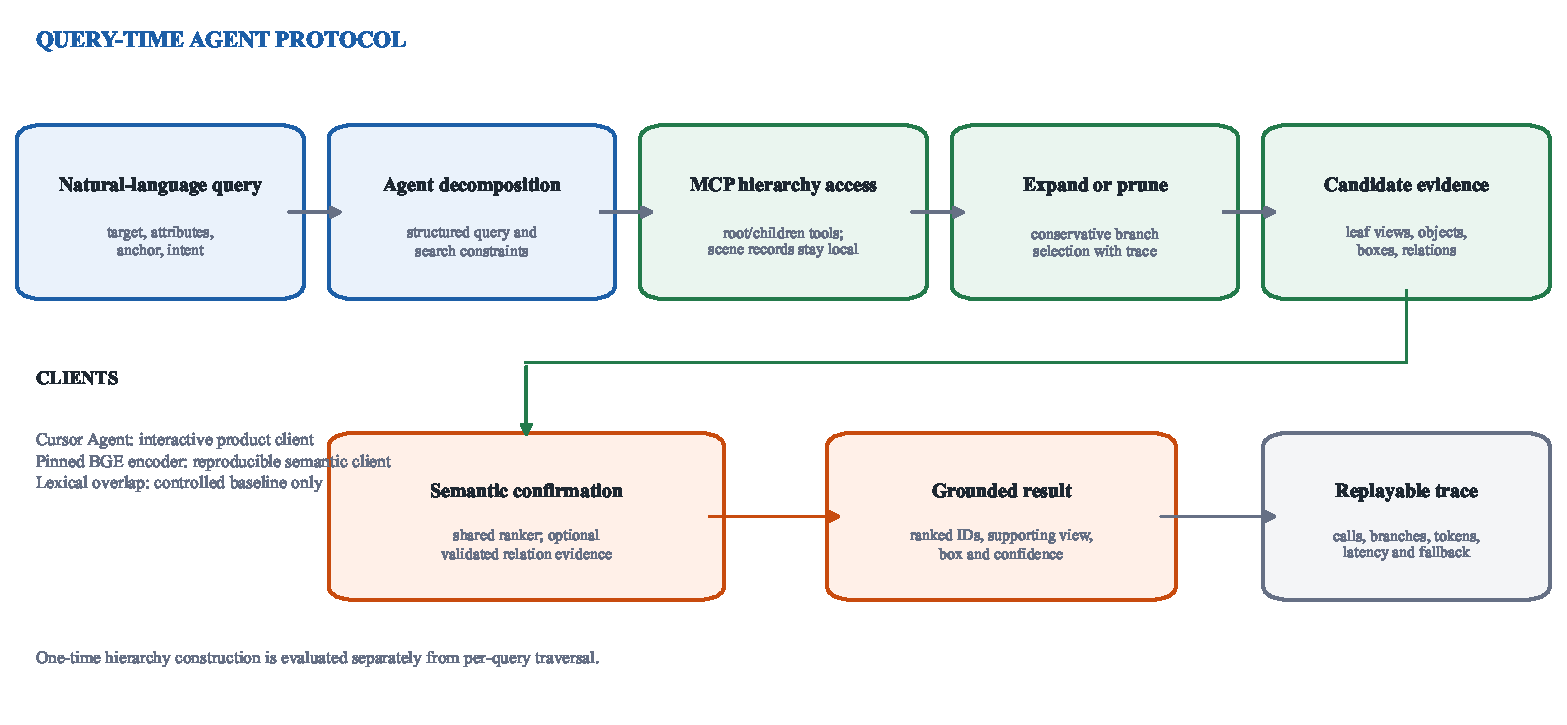
\includegraphics[width=0.98\textwidth]{figures/fig_agent_mcp_protocol.pdf}
\caption{\method. The agent decomposes a query, reads local hierarchy nodes
through MCP, expands or prunes branches, validates leaf evidence, and writes a
replayable trace. Cursor Agent is the interactive client; the pinned local
encoder supplies the reproducible semantic client. One-time hierarchy
construction is evaluated separately.}
\label{fig:agent-protocol}
\end{figure*}

\subsection{Agent--MCP Query Protocol}
Let a scene hierarchy be $H=(V,E)$ and let $\mathcal{C}$ be canonical semantic
records linked to its leaves. A query client does not receive
$\mathcal{C}$ in one prompt. It uses the following protocol:
\begin{enumerate}
  \item decompose query $q$ into target, attributes, optional anchor/relation,
  and intent;
  \item request the root and compact child summaries through MCP;
  \item select conservative child IDs to expand and record rejected siblings;
  \item retrieve candidate leaf views/objects and validate semantic or spatial
  evidence;
  \item rank stable IDs, return supporting evidence, and finalize a trace.
\end{enumerate}

The MCP server owns scene access, hierarchy inspection, geometry, and trace
persistence. The client owns semantic decisions. This boundary permits Cursor
Agent, a local model, or another compatible client without changing map
storage. The trace stores exact tool requests/responses, model identity,
branches considered, token method, latency, fallback, and final IDs.

\paragraph{Clients and controls.}
Cursor Agent is the interactive client used for direct MCP hierarchy
construction. Its UI label in this study is ``Cursor Grok 4.5 High Fast.''
Cursor did not expose auditable token usage, so those fields remain
unavailable. Reproducible query experiments use
\texttt{BAAI/bge-small-en-v1.5}, a 384-dimensional encoder run with FastEmbed
ONNX on CPU. It replaces free-form agent choices with cosine similarity while
preserving the same top-down decision boundary. It is a semantic model, not an
LLM and not evidence of Cursor quality. Lexical overlap is a non-model control.

\subsection{Hierarchy Construction}
Each captured record contains a posed view, semantic summary, objects, regions,
landmarks, attributes, relations, and optional boxes. Construction produces
scene--zone--entity--view containment edges and stable node IDs. We evaluate
four variants:
\begin{enumerate}
  \item \textbf{Manual reference}: existing human/Cursor-assisted zones;
  \item \textbf{Pose only}: deterministic camera-position clustering with
  spatial scale factor 3.5;
  \item \textbf{Pose + semantic}: pose clusters followed by deterministic
  summary-based merging;
  \item \textbf{Cursor Agent + MCP}: five direct
  \texttt{build\_spatial\_clusters} calls, followed by agent zone decisions.
\end{enumerate}

The Cursor client was not shown manual-zone labels, did not call persistence
tools, and did not modify scene data. Its five input cluster counts were
$1,1,1,2,3$ and its final hierarchy covers all 97 views without duplicate
assignment. Fixed thresholds, seed 20260724, decisions, and rationales are
released. Manual zones overlap by design, so structure agreement uses
multi-membership pairwise F1 and weighted best-zone Jaccard rather than a
single-label clustering metric.

\subsection{Semantic Records and Structured Queries}
Each searchable candidate is
\begin{equation}
c_i=(\mathrm{id}_i,\tau_i,A_i,y_i,x_i,R_i,B_i,V_i),
\label{eq:candidate}
\end{equation}
where $\tau_i$ is type, $A_i$ the ancestor path, $y_i$ label, $x_i$ searchable
text, $R_i$ typed relations, $B_i$ optional 2D/3D boxes, and $V_i$ supporting
views. Source object IDs are retained where available. Graph and flat variants
consume identical $c_i$.

A query is represented as
\begin{equation}
q=(q_t,q_a,r,\mathcal{A},\iota),
\end{equation}
with target $q_t$, anchor $q_a$, relation $r$, attributes $\mathcal{A}$, and
intent $\iota$. Intent expansion maps functional requests to candidate
affordances; for example, ``find a place to sit'' activates chair, sofa, bench,
couch, armchair, lounge, and seating records.

\subsection{Top-Down Semantic Traversal}
At node $v$, the semantic client embeds $q$ and each child summary. With cosine
scores $z_j$, it retains up to three children whose score is at least 0.20 and
within 0.08 of the best child. If no child meets the threshold, a fixed
three-child fallback is recorded. The same encoder ranks leaf evidence.
Flat-semantic search embeds all scene records without hierarchy decisions.

The lexical graph control computes branch token overlap $u_j$. If
$u_{\max}>0$, branches satisfying
\begin{equation}
u_j\geq\max(1,0.5u_{\max})
\label{eq:lexical-gate}
\end{equation}
are retained; if all overlap is zero, all branches are eligible. The identical
lexical scorer ranks retained or flat candidates. Stable-ID tie breaking keeps
the run deterministic.

\subsection{Validated Relation Reasoning}
Relations are parsed only when a target--anchor predicate and required frame
exist. Anchor confidence and margin are checked before geometry. Valid 3D
boxes are preferred; normalized 2D boxes are used only for image-frame
relations. Non-finite coordinates, non-positive extents, or absent viewpoint
frames invalidate evidence.

Relation evidence may change ranking only if confidence is at least 0.65 and
the candidate's lexical score is within 0.15 of the best lexical candidate.
Unresolved evidence triggers deterministic fallback and cannot break a lexical
tie. This prevents world-coordinate boxes from masquerading as
viewpoint-relative left/right/front/behind evidence.

\subsection{Output, Accounting, and Complexity}
Every result contains ranked IDs, supporting views/boxes, visited ancestors,
checked counts, fallback reason, runtime, serialized context, token method,
model calls, GT eligibility, and provenance. Model input tokens use the native
BGE tokenizer; lexical context uses a pinned local tokenizer. Cursor usage is
reported only when exposed. One-time construction cost is never mixed with
per-query cost.

For $N$ scene records and $N_q$ retained records, flat scoring is $O(N)$ and
graph leaf scoring is $O(N_q)$ after the hierarchy gate. Fallback has the flat
worst case. An agent may make more small calls while processing fewer total
tokens; both values are therefore reported.

\section{Datasets and Evaluation}
\subsection{Evaluation Tracks}
\begin{table*}[t]
\centering
\caption{Evaluation tracks and denominators. $Q_{\mathrm{total}}$ contributes
to cost; $Q_+$ to retrieval quality; $Q_-$ to negative accuracy; $Q_{\mathrm
{box}}$ to 3D box metrics.}
\label{tab:tracks}
\small
\tableformat
\begin{tabularx}{0.96\textwidth}{@{}lrrrrrY@{}}
\toprule
\textbf{Track} & \textbf{Scenes} & $\mathbf{Q_{\mathrm{total}}}$ &
$\mathbf{Q_+}$ & $\mathbf{Q_-}$ & $\mathbf{Q_{\mathrm{box}}}$ &
\textbf{Map/evidence type} \\
\midrule
Captured scenes & 5 & 150 & 125 & 0 & 0 &
Manual records and verified expected views \\
Replica & 8 & 56 & 48 & 8 & 48 &
Official oracle object IDs and boxes \\
ScanNet original & 8 & 48 & 48 & 0 & 48 &
Official oracle object IDs/boxes; Nr3D/Sr3D+ \\
ScanNet extended & 8 & 64 & 56 & 8 & 56 &
Original plus functional and verified-absence queries \\
ConceptGraphs native & 16 & 104 & 96 & 0 & 96 &
Predicted object maps; separate protocol \\
LangSplat native & 1 & 6 & 6 & 0 & 0 &
Learned language field; separate protocol \\
\bottomrule
\end{tabularx}
\end{table*}

\paragraph{Captured scenes.}
Five team-captured indoor/outdoor scenes contain 97 RGB-D views and 1,066
semantic items. The benchmark has 25 queries in each of six categories:
simple-object, attribute, relational, functional, multi-hop, and negative.
Verified expected views exist for 125 queries. The remaining 25 negative
queries contribute to cost only because no independent negative GT exists.

\paragraph{Public oracle-map tracks.}
The BBQ-aligned Replica subset contains 575 official object boxes. The ScanNet
subset contains 392 official boxes and 48 mapped Nr3D/Sr3D+ queries. The
extended ScanNet track adds one GT-backed functional query and one
verified-absence query per scene. These tracks evaluate retrieval over known
objects, not automatic segmentation or map construction.

\paragraph{Native predicted-map tracks.}
ConceptGraphs constructs predicted maps for all eight selected ScanNet and
eight Replica scenes. LangSplat executes RGB 3DGS optimization, SAM/CLIP
preprocessing, autoencoder compression, language-field optimization,
rendering, and six queries on ScanNet 0011\_00. Different map construction and
resource profiles keep these executions outside the oracle-map ranking.

\subsection{Metrics and Statistical Protocol}
For each method/query we record views $V$, objects $O$, nodes $G$, elapsed time
$t$, context characters $C$, input tokens $T$, and model calls. Ratio-of-sums
reduction against flat is
\begin{equation}
\Delta_X=100\left(1-\frac{\sum_qX_{gq}}{\sum_qX_{fq}}\right)\%.
\end{equation}
This definition yields 75.43\% fewer views for lexical graph traversal and
75.4\% when rounded to one decimal.

For ranked expected views or objects we report hit/Recall@$k$ and reciprocal
rank. A 3D prediction is scored with
\begin{align}
\mathrm{IoU}_{3D}&=\frac{|B_p\cap B_g|}{|B_p\cup B_g|},\\
\acc@\tau&=\frac{1}{|Q_{\mathrm{box}}|}
\sum_q\mathbf{1}[\mathrm{IoU}_{3D}\geq\tau].
\end{align}
Eligible misses score zero. Segmentation mIoU is unavailable without paired
predicted and reference point labels. Paired differences use 10,000 query
bootstrap resamples with seed 20260715.

\begin{table*}[t]
\centering
\caption{Metric prerequisites and denominators. Missing evidence remains
unavailable rather than becoming zero.}
\label{tab:metric-contract}
\footnotesize
\tableformat
\setlength{\tabcolsep}{5pt}
\begin{tabularx}{0.96\textwidth}{@{}
  >{\raggedright\arraybackslash}p{0.17\textwidth}
  >{\raggedright\arraybackslash}p{0.24\textwidth}
  >{\raggedright\arraybackslash}p{0.24\textwidth}
  Y@{}}
\toprule
\textbf{Metric} & \textbf{Prediction requirement} &
\textbf{Reference requirement} & \textbf{Denominator} \\
\midrule
\multicolumn{4}{@{}l}{\textit{Efficiency and cost}} \\
\addlinespace[3pt]
Checked views/objects/nodes & Traversal trace & None & All completed queries \\
Runtime and usage & Timed result and count metadata & None &
Results with that measurement \\
\addlinespace[5pt]
\multicolumn{4}{@{}l}{\textit{Retrieval quality}} \\
\addlinespace[3pt]
hit@$k$ & Ranked view IDs & Verified expected view IDs &
Eligible positive-view queries \\
Recall@$k$, MRR & Ranked object IDs & Official expected object IDs &
Object-ID-eligible positive queries \\
Negative accuracy & Explicit not-found result & Verified object absence &
Verified negative queries \\
\addlinespace[5pt]
\multicolumn{4}{@{}l}{\textit{Geometry and segmentation}} \\
\addlinespace[3pt]
3D IoU, Acc@$\tau$ & Valid predicted 3D box & Valid official 3D box &
Box-eligible queries; misses score zero \\
Segmentation mIoU & Predicted point labels & Paired GT segmentation &
Paired points/classes only \\
\bottomrule
\end{tabularx}
\end{table*}

\section{Experiments}
\subsection{Four Query Variants}
\begin{figure*}[t]
\centering
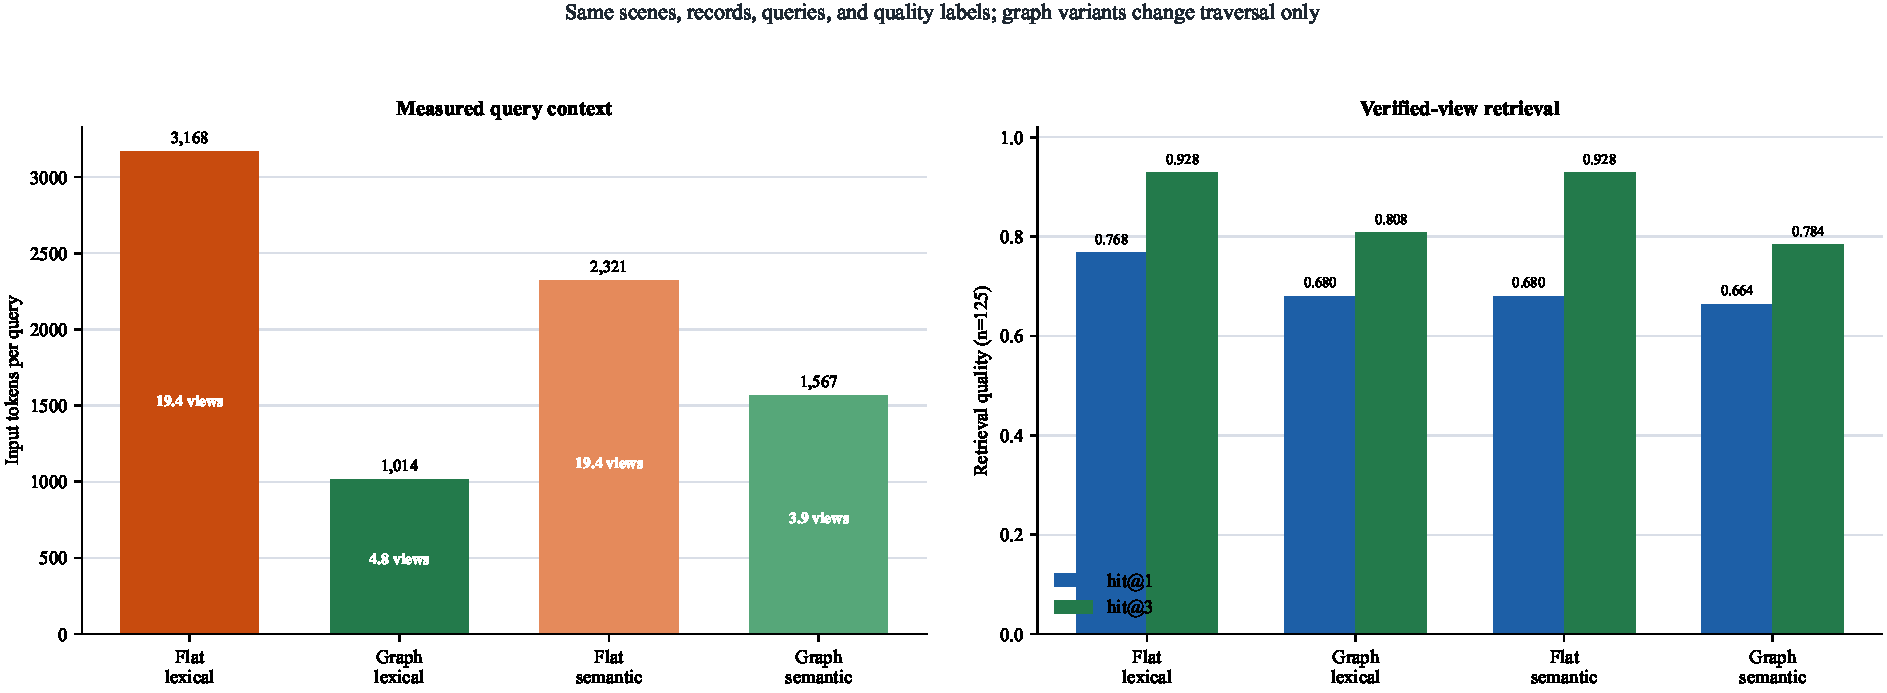
\includegraphics[width=0.96\textwidth]{figures/fig_agent_semantic_results.pdf}
\caption{Four query variants over identical scenes, records, queries, and
quality labels. Semantic tokens use the model's native tokenizer; lexical
tokens count serialized inspected context.}
\label{fig:query-variants}
\end{figure*}

\begin{table*}[t]
\centering
\caption{Same-input query benchmark. Quality uses $Q_+=125$; cost uses
$Q_{\mathrm{total}}=150$. Runtime includes local model execution where
applicable.}
\label{tab:query-variants}
\small
\tableformat
\begin{tabular}{@{}lrrrrrrrrr@{}}
\toprule
\textbf{Method} & \textbf{hit@1} & \textbf{hit@3} & \textbf{MRR} &
\textbf{Obj. hit} & \textbf{Views} & \textbf{Tokens} & \textbf{ms} &
\textbf{Calls} & \textbf{Total tokens} \\
\midrule
\tableinput{tables/agent_variant_rows.tex}
\bottomrule
\end{tabular}
\end{table*}

Lexical graph reduces views by 75.43\% and input tokens by 67.99\%. Its
graph-minus-flat hit@1 difference is $-0.088$ with 95\% CI
$[-0.184,0.008]$, which is inconclusive. The hit@3 difference is $-0.120$
with CI $[-0.184,-0.056]$, a significant decline.

Semantic graph reduces views by 79.90\% and native input tokens by 32.50\%.
Mean per-query token reduction is 32.73\% with CI $[27.11,38.21]$. The hit@1
difference is $-0.016$ with CI $[-0.096,0.064]$ and is inconclusive. The
hit@3 difference is $-0.144$ with CI $[-0.224,-0.072]$; MRR differs by
$-0.082$ with CI $[-0.150,-0.016]$. Thus the frozen semantic gate saves
context and CPU time but does not preserve top-3 quality.

Graph-semantic execution makes more small encoder calls because it scores
successive hierarchy levels. This is why call count and processed tokens are
reported separately. Model load is 9.459\,s; observed process RSS after load is
212.88\,MB and peak observed RSS is 471.00\,MB.

\subsection{Hierarchy Construction}
\begin{figure*}[t]
\centering
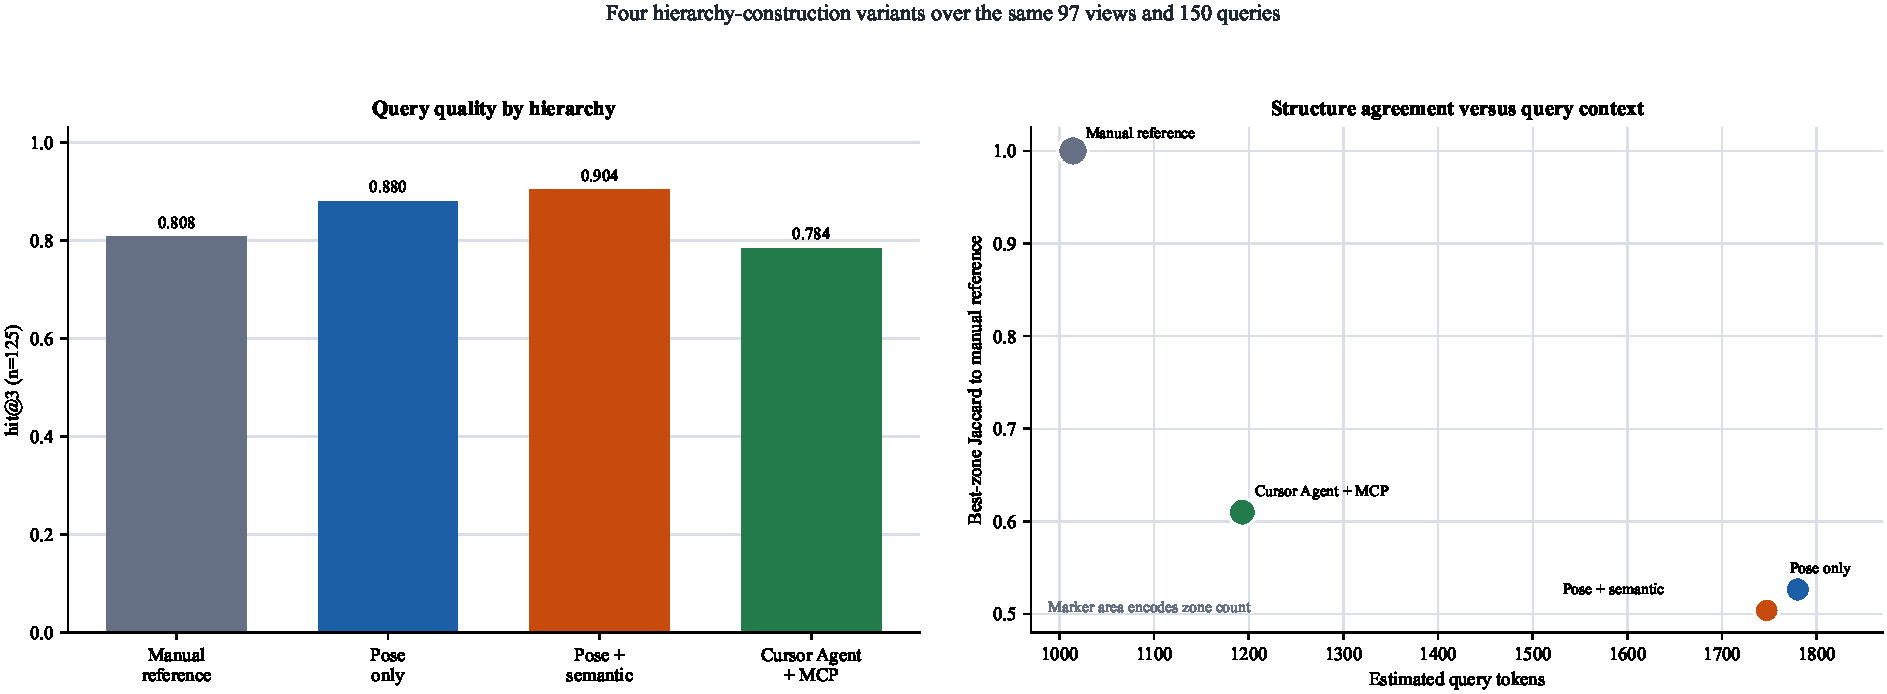
\includegraphics[width=0.96\textwidth]{figures/fig_hierarchy_comparison.pdf}
\caption{Hierarchy construction changes grouping and therefore query behavior,
but not underlying semantic records. Manual agreement is a project reference,
not independent GT.}
\label{fig:hierarchy-results}
\end{figure*}

\begin{table*}[t]
\centering
\caption{Hierarchy construction on the same 97 views and 150 queries.
Agreement compares to overlapping manual zones; quality uses $n=125$.}
\label{tab:hierarchy}
\small
\tableformat
\begin{tabular}{@{}lrrrrrrrrr@{}}
\toprule
\textbf{Hierarchy} & \textbf{Zones} & \textbf{Pair F1} &
\textbf{Jacc.} & \textbf{hit@1} & \textbf{hit@3} & \textbf{MRR} &
\textbf{Views} & \textbf{Tokens} & \textbf{Build s} \\
\midrule
\tableinput{tables/hierarchy_rows.tex}
\bottomrule
\end{tabular}
\end{table*}

Pose-plus-semantic gives the highest hit@$k$ in this experiment. Cursor--MCP is
structurally closer to the manual reference than either deterministic
alternative and uses less query context, but does not dominate their quality.
The correct claim is therefore \emph{agent-assisted hierarchy construction},
not fully automatic construction.

All deterministic variants consume zero provider tokens. Historical manual
time and Cursor UI runtime/token usage are unavailable, not zero. Each variant
has 8,939 locally estimated serialized input-context tokens. The Cursor result
is supported by five direct MCP calls and saved rationales; it is not inferred
from the manual hierarchy.

\subsection{Public Oracle-Map Protocols}
\begin{table*}[t]
\centering
\caption{Public oracle-map results. Replica is a lexical sanity ceiling.
ScanNet original and extended are discriminative. Tokens are local context
estimates, not provider billing.}
\label{tab:public}
\footnotesize
\tableformat
\setlength{\tabcolsep}{3.8pt}
\begin{tabular}{@{}llrrrrrrrr@{}}
\toprule
\textbf{Track} & \textbf{Method} & \textbf{R@1} & \textbf{R@3} &
\textbf{R@5} & \textbf{MRR} & \textbf{A@.25} & \textbf{Neg.} &
\textbf{Objects} & \textbf{Tokens} \\
\midrule
\tableinput{tables/public_rows.tex}
\bottomrule
\end{tabular}
\end{table*}

Replica quality saturates because the oracle labels are lexically easy. It is
a sanity check, not evidence that variants are equivalent generally.
Graph+fallback preserves the flat lexical ceiling while checking 27.9\% fewer
objects.

On original ScanNet, graph+fallback exactly preserves flat lexical R@1, R@3,
R@5, MRR, and Acc@0.25 while checking 25.0\% fewer objects and using 24.9\%
fewer estimated tokens. Aggressive graph search checks 90.3\% fewer objects but
loses 2.1 points at R@1, R@3, and R@5. On extended ScanNet, fallback again
preserves flat values with 18.8\% fewer objects and 18.7\% fewer tokens.

The extended positive denominator is 56, not 64; the remaining eight queries
measure verified negative accuracy. Its eight functional queries obtain
R@1=.625, R@3=.750, R@5=.750, and MRR=.667 under graph+fallback. Attribute
disambiguation remains weak (two queries; R@1=.000).

\subsection{Controlled Relation Audit}
The relation audit compares graph+fallback with the identical pipeline under
\texttt{no\_relation=true}. On 40 ScanNet relation-labelled queries, 35 parse
to a supported target--anchor predicate and five remain explicitly unparsed.
Validated relations increase hit@1 from .550 to .675. Exactly five top-1
changes are beneficial, zero are harmful, and all five pass the confidence and
score-margin gates. Gains comprise one \emph{between}, one \emph{closest}, and
three \emph{farthest} queries.

The prior relation underperformance arose because low-confidence evidence
could break lexical ties and frame-dependent predicates could be applied
without adequate validation. The new policy blocks both behaviors. On Replica,
eight parsed \emph{near} queries and eight sequential multi-hop prompts remain
correct with and without reranking; no top-1 result changes.

\begin{table}[t]
\centering
\caption{Controlled ScanNet relation audit ($Q=40$).}
\label{tab:relation}
\small
\tableformat
\begin{tabular}{@{}lrr@{}}
\toprule
\textbf{Measure} & \textbf{No relation} & \textbf{Validated relation} \\
\midrule
\tableinput{tables/relation_rows.tex}
\bottomrule
\end{tabular}
\end{table}

\subsection{Native External Executions}
ConceptGraphs produces predicted object maps on all 16 selected public scenes.
Its Acc@0.25 is .0625 on both dataset tracks. LangSplat records a complete native pipeline execution
and selects an expected view for four of six queries, but returns
relevance points rather than 3D boxes. Its hardware-adapted SAM-B/CLIP-B run
uses 3,000 RGB and language iterations on a 6\,GB GPU, not the original
30,000-iteration/24\,GB scale.

\begin{table}[t]
\centering
\caption{Native external execution evidence. Protocols differ from the
oracle-map experiments; this is not a leaderboard.}
\label{tab:external}
\footnotesize
\tableformat
\begin{tabular}{@{}lrrrrr@{}}
\toprule
\textbf{Execution} & \textbf{S} & \textbf{Q} & \textbf{Quality} &
\textbf{s/q} & \textbf{Tokens} \\
\midrule
\tableinput{tables/external_rows.tex}
\bottomrule
\end{tabular}
\end{table}

External token totals use each native local tokenizer and are not comparable
to character-derived context estimates or API billing. No official BBQ
execution artifact is included.

\subsection{Qualitative Trace}
For ``Find the piano,'' the released local-semantic trace records query
encoding, root scores, three retained zone branches, leaf-level scores,
supporting views, native tokens, and per-step latency. It is reloadable under
the same trace schema used by Cursor. The local trace demonstrates
reproducibility, not a Cursor query result.

\section{Discussion}
The experiments answer three separate questions. First, hierarchical traversal
reduces context for both lexical and neural semantic scorers. Second, the
current hard pruning policy does not preserve top-3 retrieval quality on the
captured-scene benchmark; calibrated fallback is therefore necessary. Third,
hierarchy construction materially affects both cost and quality. A
pose-plus-semantic hierarchy can outperform the manual reference on hit@$k$
while differing structurally, and the Cursor--MCP hierarchy trades some
quality for closer reference agreement and lower context.

Public results reinforce the need for protocol-specific wording. Replica is a
ceiling sanity check. ScanNet distinguishes aggressive pruning, calibrated
fallback, and flat search. The safe conclusion is that fallback preserves flat
lexical quality \emph{on these two frozen ScanNet protocols}, not that graph
routing universally preserves flat retrieval. Native ConceptGraphs and LangSplat
runs verify integration under predicted/learned maps but cannot establish a
ranking against oracle-map retrieval.

The controlled relation result also changes the earlier diagnosis. Relation
reasoning itself is not harmful after anchor, frame, geometry, confidence, and
margin checks. The remaining failures are unsupported language forms and
attribute ambiguity, which should be addressed by improved parsing or a
stronger instruction-tuned client rather than by weakening geometric safety.

\section{Limitations}
\begin{itemize}
  \item Cursor Agent supplies direct hierarchy-construction decisions, but the
  150-query benchmark uses a pinned embedding model rather than Cursor or an
  instruction-tuned LLM. No Cursor query-quality claim is made.
  \item Cursor UI provider tokens and wall-clock construction time were not
  exposed. They are unavailable, not zero; only serialized local input context
  is measured.
  \item Captured-scene ViewJSON and expected views are manual reference
  artifacts. Their quality can contain correlated annotation bias.
  \item The best construction variant is still agent-assisted and starts from
  manual semantic records. This paper does not establish automatic semantic
  perception.
  \item Replica and ScanNet retrieval use oracle object identities and boxes.
  Their Acc@0.25 is retrieval-over-GT-map accuracy, not predicted-map
  segmentation or localization accuracy.
  \item Semantic graph pruning significantly reduces hit@3 and MRR under the
  frozen policy. Quality-constrained calibration remains the central algorithm
  target.
  \item Native external runs differ in maps, frame sampling, output geometry,
  and resources. They are execution evidence, not fair comparative rankings.
  \item LangSplat covers one scene under a reduced-resource profile, and no
  official BBQ execution is included.
\end{itemize}

\section{Reproducibility and Release}
The release includes method and trace schemas, 600 per-query rows for the four
query variants, 300 semantic traces, four hierarchy constructions, per-query
hierarchy results, three public protocols, relation audits, run configurations,
model/checkpoint provenance, seeds, and hardware metadata. All 150 queries
finish under all four internal methods; validation reports contain zero
errors.

The semantic run records Windows 11, Python 3.13.13, FastEmbed 0.8.0,
ONNX Runtime 1.27.0, and the BGE model name. ScanNet and Replica raw files are
not redistributed; official access and import manifests are provided. Figure
scripts read the same frozen JSON checked by the paper audit.

\noindent\begin{minipage}{\linewidth}
\begin{lstlisting}[style=commandblock]
python -B -m pytest -q -p no:cacheprovider tests
python -B scripts/validate_agent_semantic_benchmark.py \
  --output outputs/agent_semantic/five_scene_four_variant_v1
python -B scripts/check_academic_paper.py
papers/beyond-proximity/build_paper.cmd
\end{lstlisting}
\end{minipage}

\section{Conclusion}
\method restores the original agent-centered idea as an explicit, auditable
MCP protocol rather than a hidden lexical heuristic. Cursor Agent is a
demonstrated interactive client and hierarchy constructor; a pinned local
semantic model provides reproducible query evidence. Across identical
five-scene inputs, hierarchy reduces lexical and semantic query context
substantially, but the significant hit@3/MRR losses show that uncalibrated hard
pruning is not yet quality preserving. Calibrated fallback preserves flat
lexical R@1/R@3/R@5/MRR on the two frozen ScanNet protocols while reducing
objects and context, and validated relations improve relational hit@1 without
harmful top-1 changes. The next scientific step is an instruction-tuned,
quality-constrained agent evaluation on predicted public maps under one shared
scene/query/resource protocol.

\balance
{\fontsize{6.3}{6.5}\selectfont
\bibliographystyle{abbrv}
\bibliography{refs}
}

\end{document}
